\chapter{Code availability}
\label{ap2}

\newpage

%%%%%%%%%%%%%%%%%%%%%%%%%%%%%%%%%%%%%%%%%%%%
\begin{table}[b]
\footnotesize 
\begin{center}
\begin{threeparttable}
\caption[Learning Parameters for Active, Continual Fine-Tuning]{
Learning parameters used for training and fine-tuning of AlexNet for AFT in our experiments. $\mu$ is the momentum, $lr_{fc8}$ is the learning rate of the weights in the last layer, $\alpha$ is the learning rate of the weights in the rest layers, and $\gamma$ determines how $lr$ decreases over epochs. ``Epochs" indicates the number of epochs used in each step. For ACFT, all the parameters are set to the same as AFT except the learning rate $lr$, which is set to 1/10 of that for AFT.}
\label{ap2:tab:hyperparameter}
\begin{tabular}{p{0.38\textwidth}P{0.09\textwidth}P{0.09\textwidth}P{0.09\textwidth}P{0.09\textwidth}P{0.09\textwidth}}
\hline
Applications & $\mu$ & $lr$ & $lr_{fc8}$ & $\gamma$ & epoch \\
\hline
Colonoscopy frame classification & 0.9 & 1e-4 & 1e-3 & 0.95 & 8 \\
Polyp detection & 0.9 & 1e-4 & 1e-3 & 0.95 & 10 \\
Pulmonary embolism detection & 0.9 & 1e-3 & 1e-2 & 0.95 & 5 \\
\hline
\end{tabular}
\end{threeparttable}
\end{center}
\end{table}
%%%%%%%%%%%%%%%%%%%%%%%%%%%%%%%%%%%%%%%%%%%%

\section*{Active Continual Fine-tuning}
We have investigated the effectiveness of ACFT in four applications: scene classification, colonoscopy frame classification, polyp detection, and pulmonary embolism (PE) detection. Ablation studies have been conducted to confirm the significant design of our majority selection and randomization, built upon conventional entropy and diversity based active selection criteria.
For all four applications, we set $\alpha$ to 1/4 and $\omega$ to 5.
The deep learning library Matlab and Caffe are utilized to implement active learning and transfer learning (more details can be found at \href{https://github.com/MrGiovanni/Active-Learning}{https://github.com/MrGiovanni/Active-Learning}). We based our experiments on AlexNet and GoogLeNet because their architectures offer an optimal depth balance, deep enough to investigate the impact of ACFT and AFT on pre-trained CNN performance, but shallow enough to conduct experiments quickly. The learning parameters used for training and fine-tuning of AlexNet in our experiments are summarized in \tableautorefname~\ref{ap2:tab:hyperparameter}. The Adam optimizer is utilized to optimize the objective functions described in our paper. The batch size is 512 in the learning procedure.

\section*{UNet++}

Our experiments are implemented in Keras with Tensorflow backend. We use {\em early-stop} mechanism on the validation set to avoid over-fitting and evaluate the results using Dice-coefficient and Intersection over Union (IoU). Adam is used as the optimizer with a learning rate of 3$e$-4. Both UNet+ and UNet++ are constructed from the original U-Net architecture. All the experiments are performed using three NVIDIA TITAN X (Pascal) GPUs with 12 GB memory each. To facilitate reproducibility and model reuse, we have released the implementation of U-Net, UNet+, and UNet++ for various traditional and modern backbone architectures at \href{https://github.com/MrGiovanni/UNetPlusPlus}{https://github.com/MrGiovanni/UNetPlusPlus}. 


\section*{Models Genesis}

\textit{Pre-training Models Genesis:} Our Models Genesis are pre-trained from 623 Chest CT scans in LUNA~2016~\citep{setio2017validation} in a self-supervised manner. The reason that we decided not to use all 888 scans provided by this dataset was to avoid test-image leaks between proxy and target tasks, so that we can confidently use the rest of the images solely for testing Models Genesis as well as the target models, although Models Genesis are trained from only unlabeled images, involving no annotation shipped with the dataset. We first randomly crop sub-volumes, sized $64\times 64\times 32$ pixels, from different locations. To extract more informative sub-volumes for training, we then intentionally exclude those which are empty (air) or contain full tissues. Our Models Genesis 2D are self-supervised pre-trained from LUNA~2016~\citep{setio2017validation} and ChestX-ray14~\citep{wang2017chestx} using 2D CT slices in an axial view and X-ray images, respectively. For all proxy tasks and target tasks, the raw image intensities were normalized to the $[0,1]$ range before training. We use the mean square error (MSE) between input and output images as objective function for the proxy task of image restoration. As suggested by~\citet{pathak2016context} and \citet{chen2019self}, the MSE loss is sufficient for representation learning, although the restored images may be blurry.


When pre-training Models Genesis, we apply each of the transformations on sub-volumes with a pre-defined probability. That being said, the model will encounter not only the transformed sub-volumes as input, but also the original sub-volumes. This design offers two advantages:
\begin{itemize}
    \item First, the model must distinguish original versus transformed images, discriminate transformation type(s), and restore images if transformed. Our self-supervised learning framework, therefore, results in pre-trained models that are capable of handling versatile tasks.
    \item Second, since original images are presented in the proxy task, the semantic difference of input images between the proxy and target task becomes smaller. As a result, the pre-trained model can be transferable to process regular/normal images in a broad variety of target tasks.
\end{itemize}


\textit{Fine-tuning Models Genesis:} The pre-trained Models Genesis can be adapted to new imaging tasks through transfer learning or fine-tuning. There are three major transfer learning scenarios: (1) employing the encoder as a fixed feature extractor for a new dataset and following up with a linear classifier (\eg Linear SVM or Softmax classifier), (2) taking the pre-trained encoder and appending a sequence of fully-connected (\textit{fc}) layers for target classification tasks, and (3) taking the pre-trained encoder and decoder and replacing the last layer with a $1\times 1\times 1$ convolutional layer for target segmentation tasks. For scenarios (2) and (3), it is possible to fine-tune all the layers of the model or to keep some of the earlier layers fixed, only fine-tuning some higher-level portion of the model. We have evaluated the performance of our self-supervised representation for transfer learning by fine-tuning all layers in the network. In the following, we examine Models Genesis on five distinct medical applications, covering classification and segmentation tasks in CT and MRI images with varying levels of semantic distance from the source (Chest CT) to the targets in terms of organs, diseases, and modalities (see \tablename~\ref{ch5:tab:distance}) for investigating the transferability of Models Genesis.


\textit{Benchmarking Models Genesis:} For a thorough comparison, we used three different techniques to randomly initialize the weights of models: (1) a basic random initialization method based on Gaussian distributions, (2) a method commonly known as Xavier, which was suggested in~\citet{glorot2010understanding}, and (3) a revised version of Xavier called MSRA, which was suggested in~\citet{he2015delving}. They are implemented as \texttt{uniform}, \texttt{glorot\_uniform}, and \texttt{he\_uniform}, respectively, following the Initializers\footnote{\label{foot:Initializer}Initializers: \href{http://faroit.com/keras-docs/1.2.2/initializations/}{faroit.com/keras-docs/1.2.2/initializations}} in Keras. We compare Models Genesis with Rubik's cube~\citep{zhuang2019self}, the most recent multi-task and self-supervised learning method for 3D medical imaging. Considering that most of the self-supervised learning methods are initially proposed and implemented in 2D, we have extended five most representative ones~\citep{vincent2010stacked,pathak2016context,noroozi2016unsupervised,chen2019self,caron2018deep} into their 3D versions for a fair comparison (see detailed implementation in~\ref{sec:baseline_implementation_appendix}). To promote the 3D self-supervised learning research, we make our own implementation of the 3D extended methods and their corresponding pre-trained weights publicly available as an open-source tool that can effectively be used out-of-the-box. In addition, we have examined publicly available pre-trained models for 3D transfer learning in medical imaging, including NiftyNet\footnote{\label{foot:NiftyNet}NiftyNet Model Zoo: \href{https://github.com/NifTK/NiftyNetModelZoo}{github.com/NifTK/NiftyNetModelZoo}}~\citep{gibson2018niftynet}, MedicalNet\footnote{\label{foot:MedicalNet}MedicalNet: \href{https://github.com/Tencent/MedicalNet}{github.com/Tencent/MedicalNet}}~\citep{chen2019med3d}, and, the most influential 2D weights initialization, Models ImageNet. We also fine-tune I3D\footnote{\label{foot:I3D}I3D: \href{https://github.com/deepmind/kinetics-i3d}{github.com/deepmind/kinetics-i3d}}~\citep{carreira2017quo} in our five target tasks because it has been shown to successfully initialize 3D models for lung nodule detection in~\citet{ardila2019end}. The detailed configurations of these models can be found in \ref{sec:public_3d_model_appendix}.

3D U-Net architecture\footnote{\label{foot:3dunet}3D U-Net: \href{https://github.com/ellisdg/3DUnetCNN}{github.com/ellisdg/3DUnetCNN}} is used in 3D applications; U-Net architecture\footnote{\label{foot:densenet121}Segmentation Models: \href{https://github.com/qubvel/segmentation_models}{github.com/qubvel/segmentation\_models}} is used in 2D applications. Batch normalization~\citep{ioffe2015batch} is utilized in all 3D/2D deep models. For proxy tasks, SGD method~\citep{zhang2004solving} with an initial learning rate of $1e0$ is used for optimization. We use \texttt{ReduceLROnPlateau} to schedule learning rate, in which if no improvement is seen in the validation set for a certain number of epochs, the learning rate is reduced. For target tasks, Adam method~\citep{kinga2015method} with a learning rate of $1e-3$ is used for optimization, where $\beta_1=0.9$, $\beta_2=0.999$, $\epsilon=1e-8$. We use \textit{early-stop} mechanism on the validation set to avoid over-fitting. Simple yet heavy 3D data augmentation techniques are employed in all five target tasks, including random flipping, transposing, rotating, and adding Gaussian noise. We run each method ten times on all of the target tasks and report the average, standard deviation, and further present statistical analysis based on an independent two-sample \textit{t}-test.

In the proxy task, we pre-train the model using 3D sub-volumes sized $64\times 64\times 32$, whereas in target tasks, the input is not limited to sub-volumes with certain size. That being said, our pre-trained models can be fine-tuned in the tasks with CT sub-volumes, entire CT volumes, or even MRI volumes as input upon user's need. The flexibility of input size is attributed to two reasons: (1) our pre-trained models learn generic image representation such as appearance, texture, and context feature, and (2) the encoder-decoder architecture is able to process images with arbitrary sizes.

\section*{Implementation Details of Revised Baselines}
\label{sec:baseline_implementation_appendix}


This work is among the first effort to create a comprehensive benchmark for existing self-supervised learning methods for 3D medical image analysis. We have extended the six most representative self-supervised learning methods into their 3D versions, including De-noising~\citep{vincent2010stacked}, In-painting~\citep{pathak2016context}, Jigsaw~\citep{noroozi2016unsupervised}, and Patch-shuffling~\citep{chen2019self}. These methods were originally introduced for the purpose of 2D imaging. 
On the other hand, the most recent 3D self-supervised method~\citep{zhuang2019self} learns representation by playing a Rubik's cube.
We have reimplemented it because their official implementation is not publicly available at the time this dissertation is written. All of the models are pre-trained using the LUNA~2016 dataset~\citep{setio2017validation} with the same sub-volumes extracted from CT scans as our models (see \tablename~\ref{ch5:tab:terminology}). The detailed implementations of the baselines are elaborated in the following sections.

\textit{Extended 3D De-noising:} In our 3D De-noising, which is inspired by its 2D counterpart~\citep{vincent2010stacked}, the model is trained to restore the original sub-volume from its transformed one with additive Gaussian noise (randomly sampling $\sigma\in[0,0.1]$). To correctly restore the original sub-volume, models are required to learn Gabor-like edge detectors when denoising transformed sub-volumes. Following the proposed image restoration training scheme, the auto-encoder network is replaced with a 3D U-Net, wherein the input is a $64\times 64\times 32$ sub-volume that has undergone Gaussian noise and the output is the restored sub-volume. The L2 distance between input and output is used as the loss function. 

\begin{figure*}[t]
\begin{center}
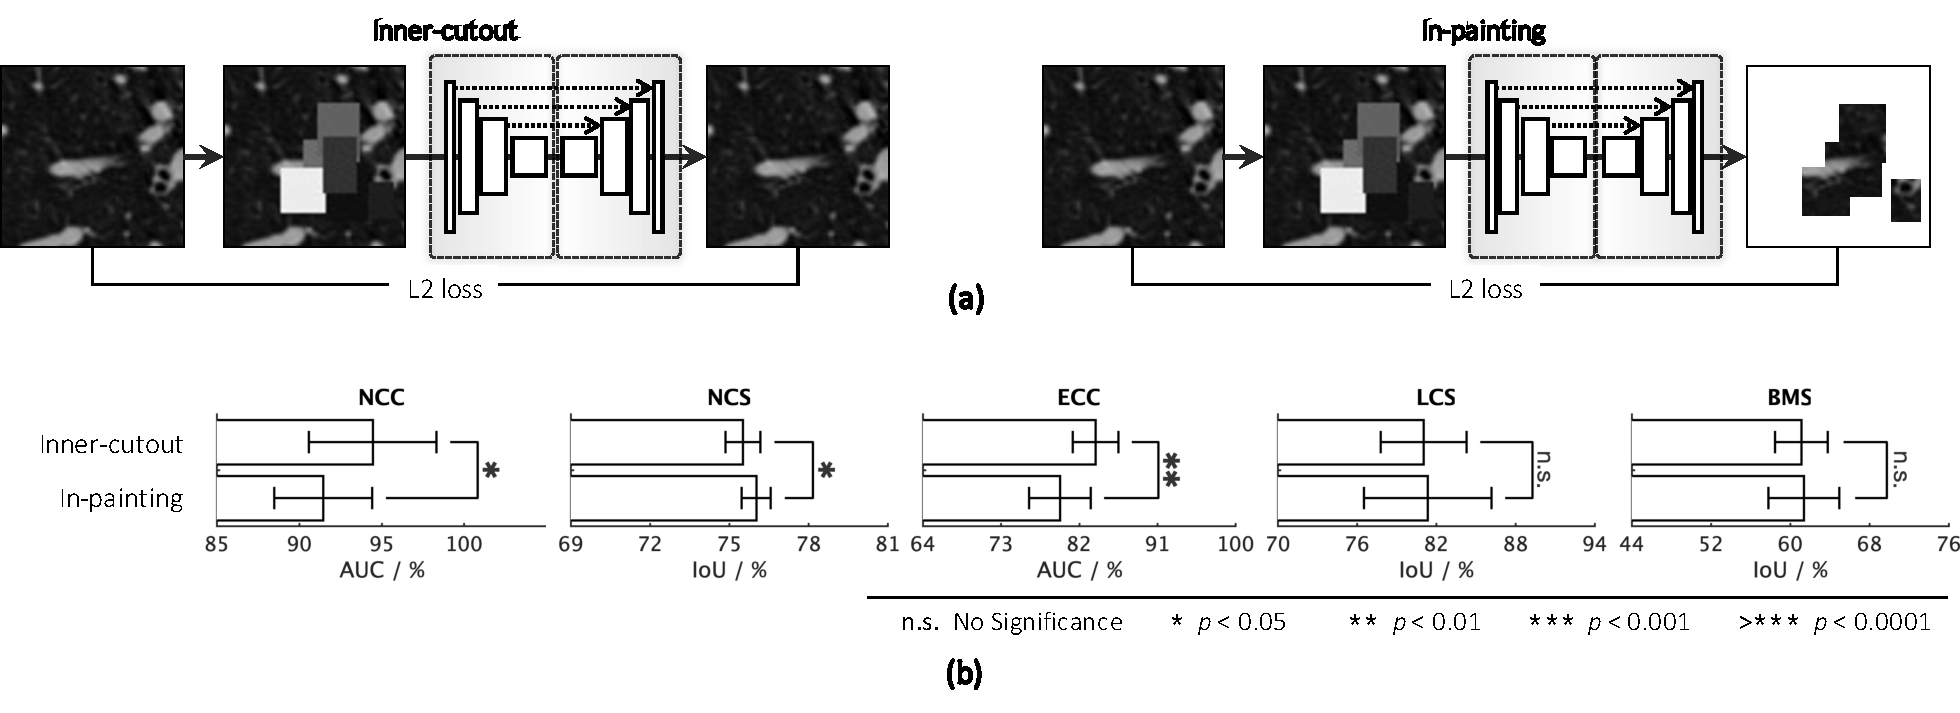
\includegraphics[width=1.0\linewidth]{Figures/AP2/fig_innercutout_inpainting.pdf}
\end{center}
\caption[Comparison Between Image In-painting and Inner-cutout]{
A direct comparison between image in-painting~\citep{pathak2016context} and our inner-cutout. (a) contrasts our inner-cutout with in-painting, wherein the model in the former scheme computes loss on the entire image and the model in the latter scheme computes loss only for the cutout area. (b) presents the performance on five target tasks, showing that inner-cutout is better suited for target classification tasks (\eg \texttt{NCC} and \texttt{ECC}), while in-painting is more helpful for target segmentation tasks (\eg \texttt{NCS}, \texttt{LCS}, and \texttt{BMS}).
}
\label{ap2:fig:innercutout_inpainting}
\end{figure*}

\textit{Extended 3D In-painting:} In our 3D In-painting, which is inspired by its 2D counterpart~\citep{pathak2016context}, the model is trained to in-paint arbitrary cutout regions based on the rest of the sub-volume. A qualitative illustration of the image in-painting task is shown in the right panel of \figurename~\ref{ap2:fig:innercutout_inpainting}(a). To correctly predict missing regions, networks are required to learn local continuities of organs in medical images via interpolation. Unlike the original in-painting, the adversarial loss and discriminator are excluded from our implementation of the 3D version because our primary goal is to empower models with generic representation, rather than generating sharper and realistic sub-volumes. The generator is a 3D U-Net, consisting of an encoder and a decoder. The input of the encoder is a $64\times 64\times 32$ sub-volume that needs to be in-painted. 
Their decoder works differently than our inner-cutout because it predicts the missing region only, and therefore, the loss is just computed on the cutout region---an ablation study on the loss has been further presented in \figurename~\ref{ap2:fig:innercutout_inpainting}.


\textit{Extended 3D Jigsaw:} In our 3D Jigsaw, which is inspired by its 2D counterpart~\citep{noroozi2016unsupervised}, we utilize the implementation by~\citet{taleb20203d}\footnote{\label{foot:3d_self_learning}Self-Supervised 3D Tasks: \href{https://github.com/HealthML/self-supervised-3d-tasks}{github.com/HealthML/self-supervised-3d-tasks}}, wherein the puzzles are created by sampling a $3\times 3\times 3$ grid of 3D patches. Then, these patches are shuffled according to an arbitrary permutation, selected from a set of predefined permutations. This set with size $P=100$ is chosen out of the $(3\times 3\times 3)!$ possible permutations, by following the Hamming distance based algorithm, and each permutation is assigned an index. As a result, the problem is cast as a $P$-way classification task, \ie the model is trained to recognize the applied permutation index, allowing us to solve the 3D puzzles efficiently. We build the classification model by taking the encoder of 3D U-Net and appending a sequence of $fc$ layers. In the implementation, we minimize the cross-entropy loss of the list of extracted puzzles.


\begin{figure}[t]
\begin{center}
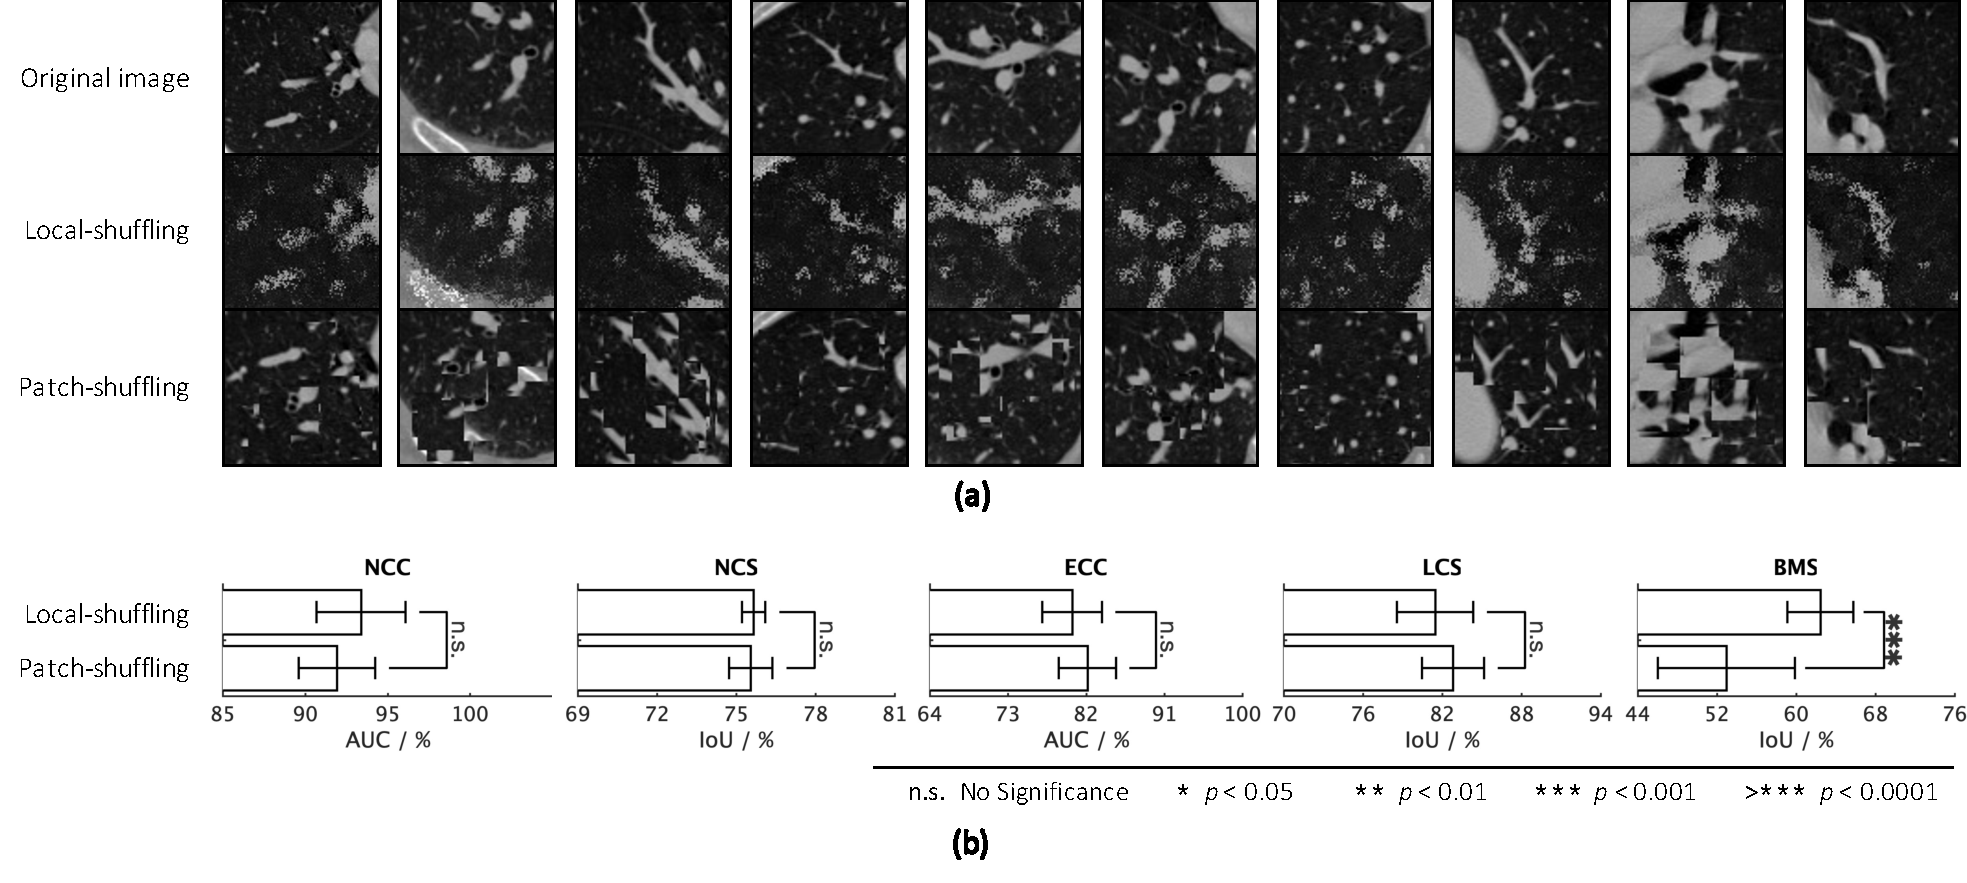
\includegraphics[width=1.0\linewidth]{Figures/AP2/fig_localshuffling_patchshuffling.pdf}
\end{center}
\caption[Comparison Between Global Patch Shuffling and Local Pixel Shuffling]{
A direct comparison between global patch shuffling~\citep{chen2019self} and our local pixel shuffling. (a) illustrates ten example images undergone local-shuffling and patch-shuffling independently. As seen, the overall anatomical structure such as individual organs, blood vessels, lymph nodes, and other soft tissue structures are preserved in the transformed image through local-shuffling.
(b) presents the performance on five target tasks, showing that models pre-trained by our local-shuffling noticeably outperform those pre-trained by patch-shuffling for cross-domain transfer learning (\texttt{BMS}). 
}
\label{ap2:fig:localshuffling_patchshuffling}
\end{figure}

\textit{Extended 3D Patch-shuffling:} In our 3D Patch-shuffling, which is inspired by its 2D counterpart~\citep{chen2019self}, the model learns image representation by restoring the image context. Given a sub-volume, we randomly select two isolated small 3D patches and swap their context. We set the length, width, and height of the 3D patch to be proportional to those in the entire sub-volume by 25\% to 50\%. Repeating this process for $T=10$ times can generate the transformed sub-volume (see examples in \figurename~\ref{ap2:fig:localshuffling_patchshuffling}(a)). The model is trained to restore the original sub-volume, where L2 distance between input and output is used as the loss function. To process volumetric input and ensure a fair comparison with other baselines, we replace their U-Net with 3D U-Net architecture, where the encoder and decoder serve as analysis and restoration parts, respectively.

\textit{Extended 3D DeepCluster:} In our 3D DeepCluster, which is inspired by its 2D counterpart~\citep{caron2018deep}, we iteratively cluster deep features extracted from sub-volumes by $k$-means and use the subsequent assignments as supervision to update the weights of the model. Through clustering, the model can obtain useful general-purpose visual features, requiring little domain knowledge and no specific signal from the inputs. We replaced original AlexNet/VGG architecture with the encoder of 3D U-Net to process 3D input sub-volumes. The number of clusters that works best for 2D tasks may not be a good choice for 3D tasks. To ensure a fair comparison, we extensively tune this hyper-parameter in $\{10,20,40,80,160,320\}$ and finally set to 260 from the narrowed down search space of $\{240,260,280\}$. Unlike ImageNet models for 2D imaging tasks, there is no available pre-trained 3D feature extractor for medical imaging tasks; therefore, we randomly initialize the model weights at the beginning. Our Models Genesis, the first generic 3D pre-trained models, could potentially be used as the 3D feature extractor and co-trained with 3D DeepCluster. 

\textit{Rubik's Cube:} We implement Rubik's Cube with respect to~\citet{zhuang2019self}, which consists of cube rearrangement and cube rotation. Like playing a Rubik's cube, this proxy task enforces models to learn translational and rotational invariant features from raw 3D data. Given a sub-volume, we partition it into a $2\times 2\times 2$ grid of cubes. In addition to predicting orders (3D Jigsaw), this proxy task permutes the cubes with random rotations, forcing models to predict the orientation. Following the original paper, we limit the directions for cube rotation, \ie only allowing 180$^{\circ}$ horizontal and vertical rotations, to reduce the complexity of the task. The eight cubes are then fed into a Siamese network with eight branches sharing the same weight to extract features. The feature maps from the last fully-connected or convolution layer of all branches are concatenated and given as input to the fully-connected layer of separate tasks, \ie cube ordering and orienting, which are supervised by permutation loss and rotation loss, respectively, with equal weights.

\section*{Configurations of Publicly Available Models}
\label{sec:public_3d_model_appendix}

For publicly available models, we do not re-train their proxy tasks and instead simply endeavor to find the best hyper-parameters for each of them in target tasks. We compare them with our Models Genesis in a user perspective, which might seem to be unfair in a research perspective because many variables are asymmetric among the competitors, such as programming platform, model architecture, number of parameters, etc. However, the goal of this section is to experiment with existing ready-to-use pre-trained models under different medical tasks; therefore, we presume that all of the publicly available models and their configurations have been carefully composed to the optimal setting.

\textit{NiftyNet:} We examine the effectiveness of fine-tuning from NiftyNet in five target tasks. We should note that NiftyNet is not initially designed for transfer learning but is one of the few publicly available supervised pre-trained 3D models. The model from~\citet{gibson2018automatic} has been considered as the baseline in our experiments because it has also been pre-trained on the chest region in CT modality and applied an encoder-decoder architecture that is similar to our work. We directly adopt the pre-trained weights of the dense V-Net architecture provided by NiftyNet, so it carries a smaller number of parameters than our 3D U-Net (2.60M vs. 16.32M). For target classification tasks, we use the dense V-Net encoder by appending a sequence of $fc$ layers; for target segmentation tasks, we use the entire dense V-Net. Since NiftyNet is developed in Tensorflow, all five target tasks are re-implemented using their build-in configuration. For each target task, we have tuned hyper-parameters (\eg learning rate and optimizer) and applied extensive data augmentations (\eg rotation and scaling).

\textit{Inflated 3D:} We download the Inflated 3D (I3D) model pre-trained from Flow streams in the Kinetics dataset~\citep{hara2018can} and fine-tune it on our five target tasks. The input sub-volume is copied into two channels to align with the required input shape. For target classification tasks, we take the pre-trained I3D and append a sequence of randomly initialized fully-connected layers. For target segmentation tasks, we take the pre-trained I3D as the encoder and expand a decoder to predict the segmentation map, resulting in a U-Net like architecture. The decoder is the same as that implemented in our 3D U-Net, consisting of up-sampling layers followed by a sequence of convolutional layers, batch normalization, and ReLU activation. Besides, four skip connections are built between the encoder and decoder, wherein feature maps before each pooling layer in the encoder are concatenated with same-scale feature maps in the decoder. All of the layers in the model are trainable during transfer learning. Adam method~\citep{kinga2015method} with a learning rate of $1e-4$ is used for optimization.

\textit{MedicalNet:} We download MedicalNet models~\citep{chen2019med3d} that have been pre-trained on eight publicly available 3D segmentation datasets. ResNet-50 and ResNet-101 backbones are chosen because they are reported by~\citet{chen2019med3d} as the most compelling backbones for target segmentation and classification tasks, respectively. Like I3D, we append a decoder at the end of the pre-trained encoder, randomly initialize its weights, and link the encoder with the decoder using skip connections. Owing to the 3D ResNet backbones, the resultant segmentation network for MedicalNet is much heavier than our 3D U-Net. To be consistent with the original programming platform of MedicalNet, we re-implement all five target tasks in PyTorch, using the same data separation and augmentation. We report the highest results achieved by any of the two backbones in \tablename~\ref{ch5:tab:top_existing_models}.